%
% Documento: Resultados
%

\chapter{Resultados}

Após a execução dos testes, foram geradas tabelas com os valores dos tempos de carregamento, desvio padrão dos tempos para cada técnica e gráficos em cascata das páginas \textit{web} desenvolvidas para cada técnica de otimização analisada. Os valores registrados mostraram as diferenças no comportamento das versões do protocolo HTTP e como cada técnica se comportaria no HTTP/2.

Neste capitulo são descritos e analisados os valores encontrados e são tiradas conclusões em cima do comportamento das páginas.

\subsection{Análise do tempo de carregamento}
\label{analisedotempodecarregamento}

O tempo de carregamento foi a métrica de desempenho escolhida para comparar o comportamento das páginas de teste nos diferentes protocolos. Essa métrica foi obtido com a ajuda da ferramenta de desenvolvedor de cada navegador. As tabelas TABELA TECNICA 1, TABELA TECNICA 2, TABELA TECNICA 3, TABELA TECNICA 4, mostram os resultados do tempo carregamento das páginas \textit{web} divididos por técnica analisada.

TABELA TECNICA 1.1

TABELA TECNICA 1.2

As TABELA TECNICA 1.1 e TABELA TECNICA 1.2 mostram os resultados obtidos com a redução de requisições HTTP concatenando arquivos CSS e JS. Diferente do esperado o HTTP/2 obteve resultados piores ou iguais ao HTTP/1.1 e ainda a concatenação dos arquivos gerou uma melhora no tempo de carregamento da página, o que não era esperado para o novo protocolo.

TABELA TECNICA 2.1

TABELA TECNICA 2.2

Analisando as TABELA TECNICA 2.1 e TABELA TECNICA 2.2 percebemos que o HTTP/2, apesar de obter desempenho melhor do que o HTTP/1.1, teve um aumento no tempo de carregamento para um número maior de CDNs. Esse aumento pode ser consequência do tempo de busca de DNS ter aumentado ou por que com as novas CDNs utilizadas possuíam desempenho ruim. Mas julgando pelo fato de todas serem CDNs grandes e muito utilizadas, devemos considerar que todas são otimizadas e possuem alto desempenho. 

TABELA TECNICA 3.1

TABELA TECNICA 3.2

As TABELA TECNICA 3.1 e TABELA TECNICA 3.2 mostram os resultados obtidos para o tempo de carregamento da página utilizando duas e três CDNs respectivamente. Mais uma vez percebe-se que o HTTP/2 possui desempenho melhor do que o HTTP/1.1 e além disso que o número de CNDs usado interfere diretamente no tempo de carregamento da página. Apesar de o resultado esperado pela análise da especificação do novo protocolo sugerir que o número de CNDs não fosse interferir no tempo de carregamento das páginas \textit{web}.

Outro motivo para isso pode ser o fato de as CDNs não suportarem requisições HTTP/2, sendo assim a comunicação com as CNDs ocorre através da versão antiga do protocolo, fato que acaba influenciando no ganho de desempenho que a página teria com o HTTP/2.

TABELA TECNICA 4.1

TABELA TECNICA 4.2

O redirecionamento não deveria influenciar no tempo de carregamento da página no HTTP/2. Apesar disso pode se perceber que quando a página é redirecionada o desempenho da mesma é pior independente do protocolo utilizado.

TABELA TECNICA 5

Na tabela TABELA TECNICA 5 encontra o resultado do tempo de carregamento da página utilizando o \textit{template} escolhido. Pode se dizer que os dois protocolos tiveram o mesmo resultado, pois as diferenças são muito pequenas. Contudo era esperado que o HTTP/2 fosse mais eficiente e carregasse a página mais rapidamente.

\subsubsection{Desvio padrão}
\label{desviopadrao}

Apesar do HTTP/2 apresentar desempenho pior ou semelhando ao HTTP/1.1 e de algumas técnicas que não deveriam alterar o comportamento do protocolo causarem terem nele um efeito não esperado, pode se notar que o novo protocolo se comporta diferente de sua versão prévia. A TABELA 6 mostra os resultados encontrados quando os desvios padrão dos tempo de carregamento de cada página testada são calculado.

TABELA 6

Observando a tabela percebe se que o HTTP/2 é um protocolo mais estável e que aparentemente sofre menos com as alterações de rede. Quando utilizando uma conexão de rede real, não é possível remover 100\% os picos e vales de conexão que ocorrem. Por esse motivo percebemos que os tempos de carregamento se alteram (apesar de os valores muito fora da média já terem sido retirados). Mesmo assim, o desvio padrão do HTTP/2 foi menor do que o do HTTP/1.1 para todas as páginas, o que pode ser uma grande vantagem para desenvolvedores tentarem prever o comportamento de seus \textit{websites} e seus usuários.

\subsubsection{Cascata}
\label{cascata}

As \autoref{fig:cascatahttp11} e \autoref{fig:cascatahttp2} mostram o carregamento do cenário \autoref{facamenosrequisicoeshttp} em formato de gráfico em cascata, obtido com a ajuda da ferramenta de desenvolvedor do Google Chrome.

\begin{figure}[!htb]
    \centering
    \caption{Cascata representando \textit{download} de componentes da página no HTTP/1.1.}
    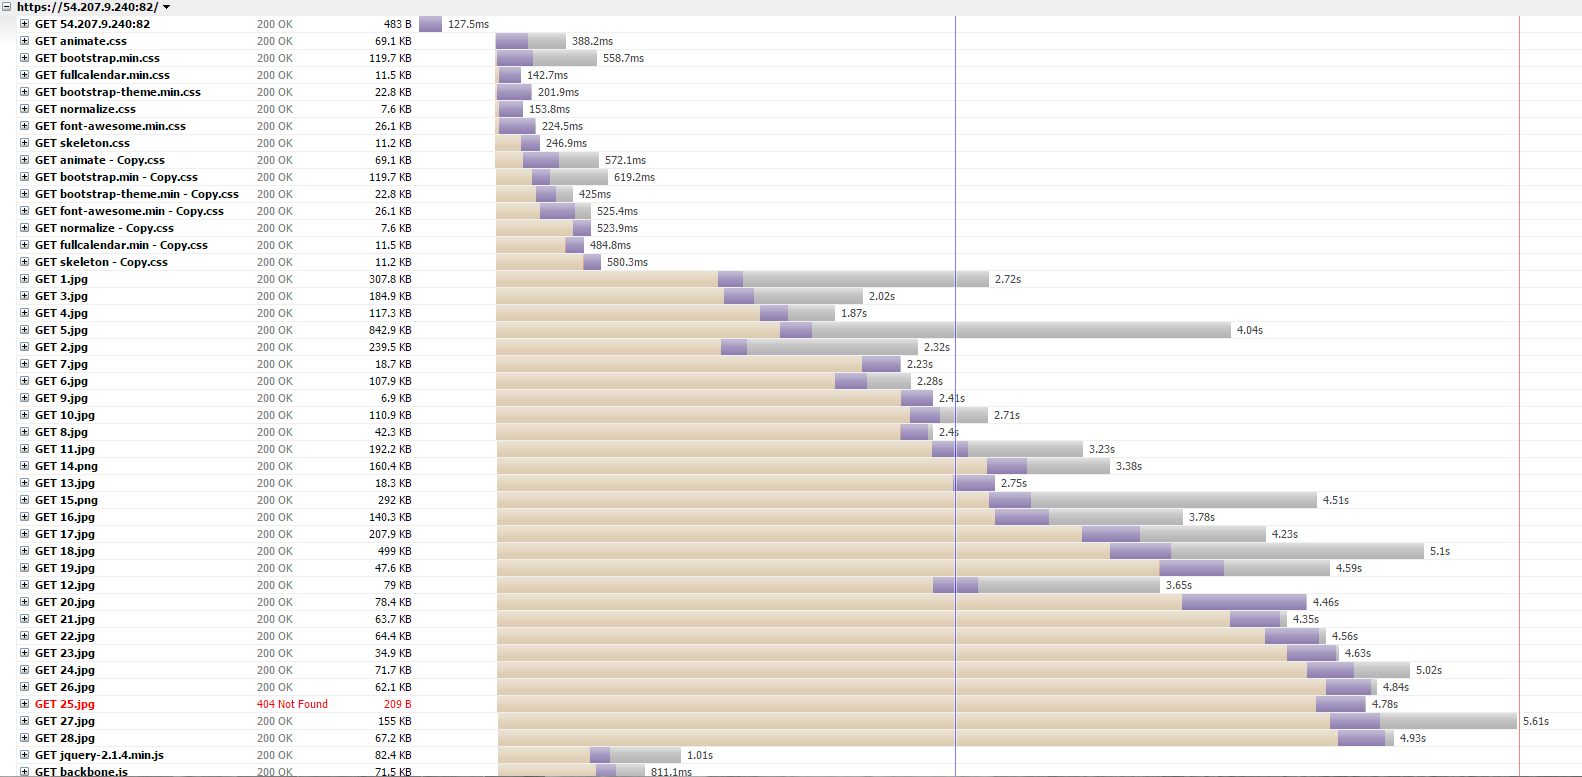
\includegraphics[width=1.0\textwidth]{./04-figuras/analise-de-resultados/cascata_http11}
    \label{fig:cascatahttp11}
\end{figure}

\begin{figure}[!htb]
    \centering
    \caption{Cascata representando \textit{download} de componentes da página no HTTP/2.}
    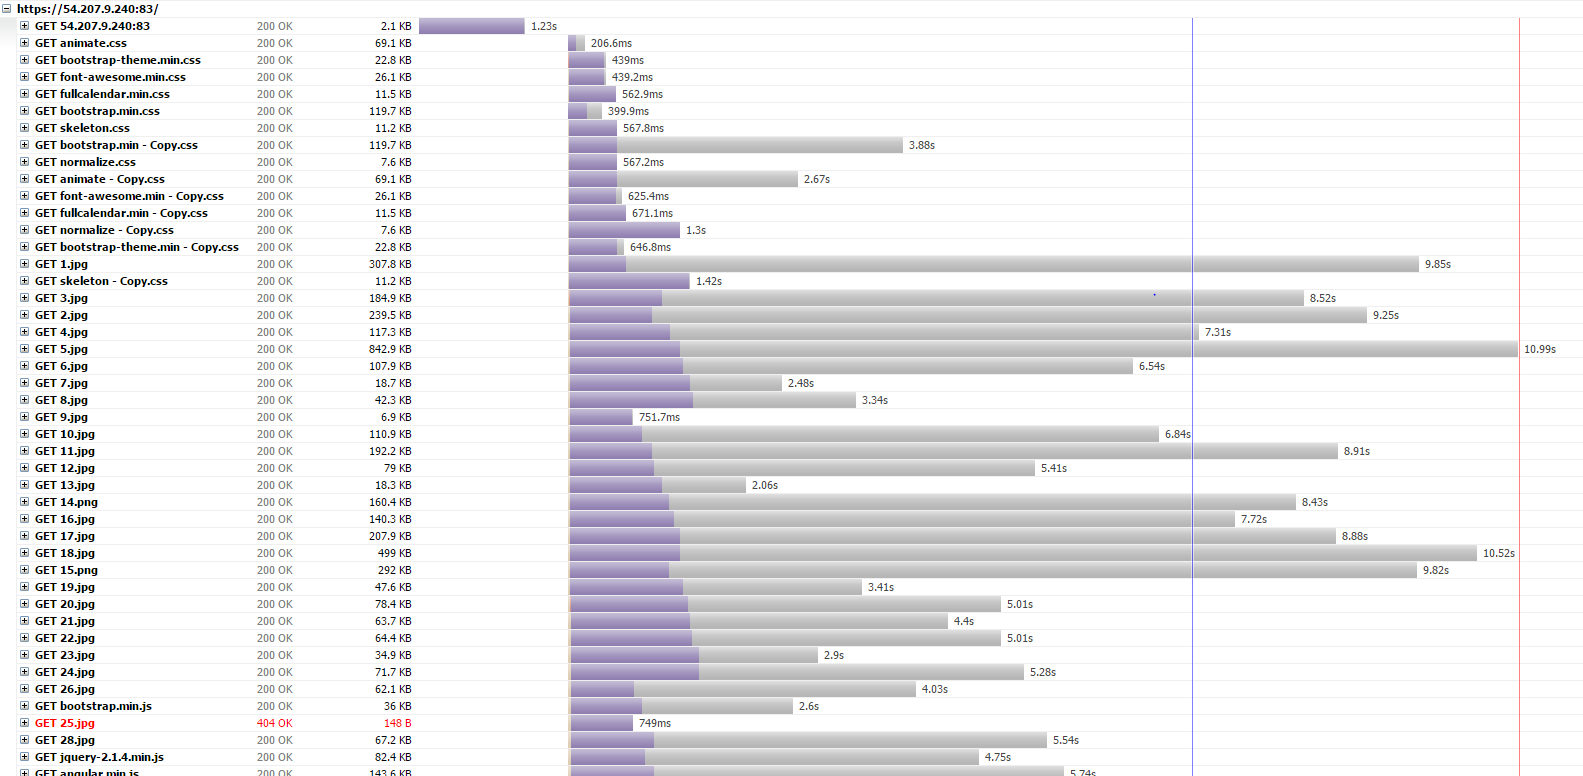
\includegraphics[width=1.0\textwidth]{./04-figuras/analise-de-resultados/cascata_http2}
    \label{fig:cascatahttp2}
\end{figure}

Nas \autoref{fig:cascatahttp11} e \autoref{fig:cascatahttp2} a cor marrom representa o tempo que o componente ficou bloqueado, ou seja, estava aguardando outros componentes serem baixados para poder começar a ser processado. Sendo assim, durante esse período nem a requisição pelo componente foi feita ainda. A porção representada pela cor roxa é o tempo que o cliente ficou esperando pelo servidor para processar sua requisição e responde-la. E a cor cinza representa o tempo de envio do componente, ou seja, o tempo que o cliente demorou para fazer o \textit{download}.

Os gráficos de cascata para os outros cenários podem ser encontrados nas FIGURA 1, FIGURA 2, FIGURA 3. Quando analisadas, essas figuras revelam a diferença no comportamento dos protocolos HTTP/1.1 e HTTP/2. Percebe se que no HTTP/1.1 os gráficos possuem o formato conhecido como cascata, onde os componentes ficam bloqueados ou não são nem processados até que outros já tenham terminado de serem baixados pelo cliente. Enquanto que no HTTP/2 a cascata não é formada, isso graças ao grande paralelismo que esse protocolo possui.

Com isso, esperava-se que o tempo gasto com componentes bloqueados no HTTP/1.1 fosse removido do tempo total de carregamento no HTTP/2. Mas podemos perceber, analisando os resultados do tempo de carregamento final das páginas, que isso não acontece. Apesar de os componentes não ficarem bloqueados, eles possuem tempo de \textit{download} muito maiores no HTTP/2.

Existem alguns fatores que podem ser a causa desse aumento no tempo de \textit{download} das páginas. Tsujikawa, desenvolvedor do \textit{ngtthp2}, acredita que um dos motivos é o fato de os navegadores não estarem preparados para utilizar todas as funcionalidades disponíveis no HTTP/2, afinal de contas o protocolo é muito novo e ainda é necessário tempo para que tal adaptação seja feita. Outros motivos que podem estar limitando os ganhos com o paralelismo do HTTP/2 são a possível falta de otimização do Nginx, que não conseguiria servir tantas requisições paralelas otimizadas ao mesmo tempo, a limitação do \textit{hardware} da máquina onde está instalado o servidor, que não possui um processador multi-tarefas, ou até mesmo limitações da rede, que possui largura de banda para transferir tantos dados ao mesmo tempo.

\subsection{Discussão dos resultados}
\label{discussaodosresultados}

A hipótese inicial deste trabalho propunha que o HTTP/2 apresentaria um desempenho melhor do que o HTTP/1.1 e que algumas técnicas de otimização de desempenho utilizadas para o protocolo mais antigo não teriam efeito ou seriam até mesmo prejudiciais para as páginas \textit{web} no novo protocolo. Mas apesar do esforço para encontrar um servidor HTTP/2 confiável e de gerar resultados que representassem o mundo real, o HTTP/2 não apresentou o comportamento esperado.

A redução de requisições HTTP continuou tendo aumentando o desempenho das páginas \textit{web}, o aumento de pesquisas de DNS foi prejudicial e o redirecionamento ainda deve ser um recurso evitado. Além disso, quando analisado em uma simulação de um site real sem sobre carga de requisições e sem a aplicação de técnicas de otimização o HTTP/2 ainda obteve resultados piores do que o HTTP/1.1.

Não foi possível analisar afundo o motivo de porque o novo protocolo não se comportou como o esperado, mas algumas perguntas ficam em aberto para serem respondidas em trabalhos futuros.

O HTTP/2 ainda está em fase de desenvolvimento e adaptação, e no decorrer dos próximos meses muitas implementações devem ser lançadas para que sejam testadas pelos usuários da \textit{Web}. Apesar de não ter obtido resultado satisfatório neste trabalho, acredita-se ainda que o novo protocolo vai ser uma grande mudança para a \textit{Web} e que as técnicas de otimização de \textit{front-end} de \textit{websites} deverão se atualizar para serem efetivas no novo protocolo.

\subsection{Questões em aberto}
\label{questoesemaberto}

A seguir encontra-se uma lista de questões deixadas em aberto por este trabalho que podem ser usadas como guias de trabalhos futuros.

\begin{itemize}
	\item Porque a implementação atual do HTTP/2 apresentou desempenho pior do que o HTTP/1.1?
	\item Quanto o \textit{hardware} da máquina onde está instalado o servidor \textit{web} interfere no desempenho do HTTP/2?
	\item O Nginx, versão 1.9.5, consegue lidar com uma grande quantidade de requisições paralelas?
	\item Os navegadores \textit{web} estão preparados para utilizar todo o potencial do HTTP/2?
	\item Porque reduzir as requisições HTTP melhorou o desempenho da página no HTTP/2?
\end{itemize}

Espera-se que as respostas para tais questões ajudem a entender o motivo dos testes deste trabalho não obterem os resultados esperados.